\chapter{Analysephase}
\label{chap:analysephase}

\section{Anforderungen}
\subsection{Funktionale Anforderungen}
Das geplante Tool soll den spezifischen Anforderungen der Zielgruppe gerecht werden und folgende Funktionen umfassen:
\begin{itemize}
    \item \textbf{Visualisierung:} Darstellung der Gesprächsdaten als Donut- und Radarcharts. Diese Diagramme ermöglichen eine schnelle Erfassung von Trends und Leistungskennzahlen und sind besonders geeignet, um die Ergebnisse von Mitarbeitendengesprächen verständlich zu präsentieren \cite{kirk2016data, evergreen2016effective}.
    \begin{figure}[h!]
    \centering
    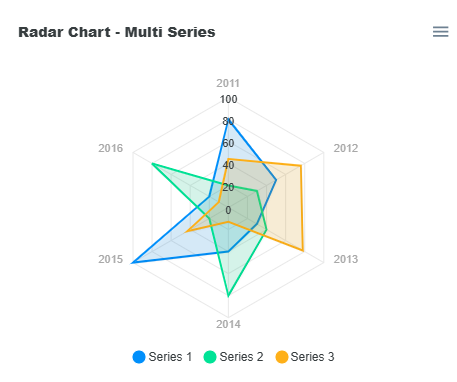
\includegraphics[width=0.8\textwidth]{images/radarchart_apexcharts.png}
    \caption{Framework Apexcharts für React}
    \label{fig:hrworks_evalea_comparison}
\end{figure}
    \item \textbf{Datenmanagement:} Import, Speicherung und Bearbeitung von Gesprächsdaten. Diese Funktion gewährleistet eine strukturierte Datenverwaltung und unterstützt die Nachverfolgbarkeit vergangener Gespräche \cite{bryson2011employee}.
    \item \textbf{Export:} Generierung von Berichten im Excel- und PDF-Format, die Führungskräfte für weitere Analysen oder Präsentationen nutzen können.
    \item \textbf{Benutzerverwaltung:} Rollenspezifischer Zugriff (z. B. Admins, Führungskräfte), um sicherzustellen, dass nur berechtigte Personen auf sensible Daten zugreifen können \cite{duarte2012performance}.
\end{itemize}

\subsection{Nicht-funktionale Anforderungen}
Neben den funktionalen Anforderungen sind nicht-funktionale Kriterien von entscheidender Bedeutung, um die Qualität und Effizienz des Tools sicherzustellen:
\begin{itemize}
    \item \textbf{Performance:} Schnelle Verarbeitung großer Datenmengen, um Wartezeiten zu minimieren.
    \item \textbf{Skalierbarkeit:} Fähigkeit, sich an wachsende Nutzer- und Datenmengen anzupassen, insbesondere in großen Organisationen.
    \item \textbf{Sicherheit:} Schutz sensibler Daten durch moderne Authentifizierungs- und Verschlüsselungsmethoden \cite{schober2008}.
\end{itemize}

\begin{table}[h!]
\centering
\caption{Zusammenfassung der funktionalen und nicht-funktionalen Anforderungen}
\label{tab:anforderungen_uebersicht}
\begin{tabularx}{\textwidth}{|X|X|}
\hline
\textbf{Anforderung}              & \textbf{Beschreibung}                                                                                                   \\\hline
Visualisierung                   & Donut- und Radarcharts zur Darstellung von Gesprächsdaten. \\\hline
Datenmanagement                  & Strukturierter Import, Speicherung und Bearbeitung von Gesprächsdaten. \\\hline
Export                           & Erstellung von Berichten im Excel- und PDF-Format. \\\hline
Benutzerverwaltung               & Rollenspezifischer Zugriff auf Gesprächsdaten. \\\hline
Performance                      & Schnelle Verarbeitung großer Datenmengen. \\\hline
Skalierbarkeit                   & Anpassungsfähigkeit an wachsende Daten- und Nutzerzahlen. \\\hline
Sicherheit                       & Schutz sensibler Daten durch Authentifizierung und Verschlüsselung. \\\hline
\end{tabularx}
\end{table}

\section{Stakeholder-Interviews und Umfragen}
\subsection{Methodik}
Zur Bedarfsanalyse wurden halbstrukturierte Interviews mit Führungskräften und HR-Managern durchgeführt. Ziel dieser Interviews war es, die spezifischen Anforderungen an das geplante Tool zu identifizieren. Die Methodik umfasste folgende Schritte:
\begin{itemize}
    \item \textbf{Teilnehmer:} Führungskräfte und HR-Manager aus verschiedenen Abteilungen.
    \item \textbf{Interviewfragen:}
    \begin{itemize}
        \item Welche Daten benötigen Sie für Ihre Entscheidungsfindung?
        \item Welche Herausforderungen bestehen bei der Nutzung bestehender Systeme?
        \item Welche Funktionen wären essenziell für Ihre tägliche Arbeit?
    \end{itemize}
    \item \textbf{Auswertung:} Qualitative Analyse der Antworten, um Muster und zentrale Anforderungen zu identifizieren.
\end{itemize}

\subsection{Ergebnisse}
Die Analyse der Interviews führte zu folgenden Erkenntnissen:
\begin{itemize}
    \item \textbf{Intuitive Diagramme:} Bedarf an einfachen Visualisierungen, die Trends und Muster in den Gesprächsdaten schnell erkennen lassen.
    \item \textbf{Echtzeit-Updates:} Wunsch nach einer Benutzeroberfläche, die Daten in Echtzeit aktualisiert.
    \item \textbf{Datensicherheit:} Hohe Anforderungen an die Vertraulichkeit und den Schutz sensibler Gesprächsdaten \cite{bryson2011employee}.
\end{itemize}

\begin{figure}[h!]
    \centering
    \includegraphics[width=0.8\textwidth]{images/stakeholder_results.png}
    \caption{Ergebnisse der Stakeholder-Analyse.}
    \label{fig:stakeholder_results}
\end{figure}

\section{Vergleich bestehender Lösungen}
\subsection{Analyse bestehender Tools}
\subsection{Vergleich von HRworks und Evalea}
Die beiden Tools \textbf{HRworks} und \textbf{Evalea} wurden hinsichtlich ihrer Funktionen und Einsatzmöglichkeiten für Mitarbeitendengespräche analysiert.

\begin{table}[h!]
\centering
\caption{Vergleich von HRworks und Evalea}
\label{tab:vergleich_hrworks_evalea}
\begin{tabularx}{\textwidth}{|X|X|X|}
\hline
\textbf{Kriterium}              & \textbf{HRworks}                                                                 & \textbf{Evalea}                                                                 \\\hline
\textbf{Visualisierung}         & Keine spezialisierte Visualisierung für Mitarbeitendengespräche.                 & Umfangreiche Reporting-Funktionen mit individuellen Gesprächsleitfäden.         \\\hline
\textbf{Datenmanagement}        & Verwaltung von Stammdaten, jedoch ohne spezifische Analysetools.                 & Strukturierte Verwaltung von Gesprächsdaten mit erweiterten Reporting-Optionen. \\\hline
\textbf{Feedback}               & Bietet 360°-Feedback-Funktionen.                                                 & Unterstützung von Feedbackprozessen für verschiedene Anlässe.                   \\\hline
\textbf{Benutzerfreundlichkeit} & Intuitive Benutzeroberfläche.                                                    & Flexibel anpassbare Gesprächsleitfäden.                                         \\\hline
\textbf{Integration}            & Integration in allgemeine HR-Prozesse wie Zeiterfassung und Abwesenheitsmanagement. & Integration mit bestehenden Systemen und maßgeschneiderten Leitfäden.          \\\hline
\end{tabularx}
\end{table}

\subsubsection{Zusammenfassung der Analyse}
\textbf{HRworks} ist eine umfassende HR-Management-Lösung, die den administrativen Aufwand reduziert und Funktionen wie Terminvereinbarung und 360°-Feedback bietet. Jedoch fehlen spezialisierte Visualisierungen für Mitarbeitendengespräche. \textbf{Evalea} zeichnet sich durch eine starke Ausrichtung auf Mitarbeitendengespräche aus, mit flexiblen Leitfäden und umfangreichen Reporting-Funktionen.

\begin{figure}[h!]
    \centering
    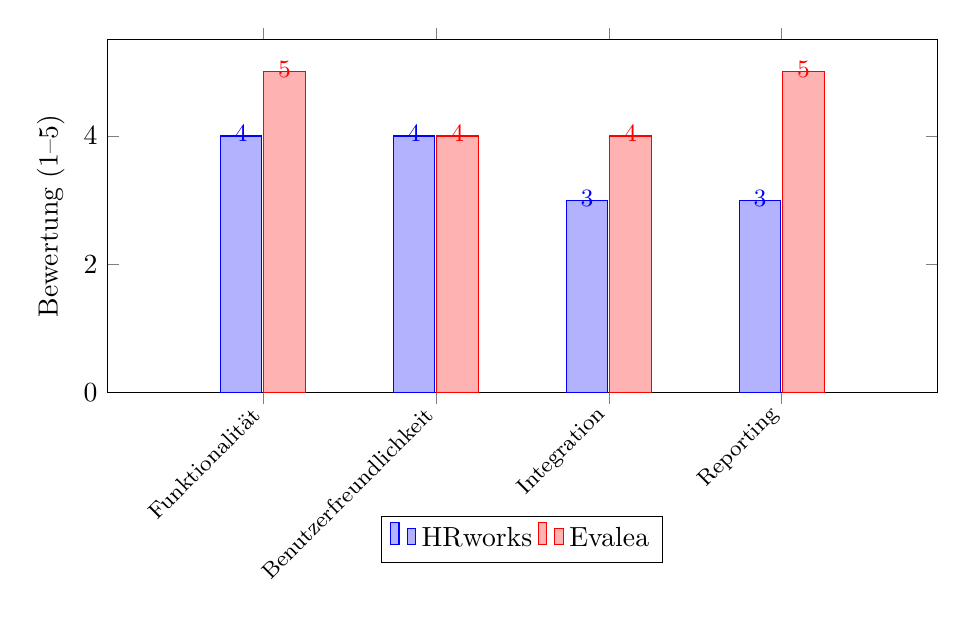
\begin{tikzpicture}
        \begin{axis}[
            width=\textwidth,
            height=0.5\textwidth,
            ybar=0.7pt,
            bar width=15pt,
            enlarge x limits=0.3,
            ylabel={Bewertung (1–5)},
            symbolic x coords={Funktionalität, Benutzerfreundlichkeit, Integration, Reporting},
            xtick=data,
            x tick label style={font=\footnotesize, rotate=45, anchor=east},
            ymin=0, ymax=5.5,
            nodes near coords,
            nodes near coords style={font=\small, anchor=mid},
            legend style={at={(0.5,-0.35)}, anchor=north, legend columns=-1},
            legend cell align={left}
        ]
        \addplot[blue,fill=blue!30] coordinates {
            (Funktionalität,4)
            (Benutzerfreundlichkeit,4)
            (Integration,3)
            (Reporting,3)
        };
        \addplot[red,fill=red!30] coordinates {
            (Funktionalität,5)
            (Benutzerfreundlichkeit,4)
            (Integration,4)
            (Reporting,5)
        };
        \legend{HRworks, Evalea}
        \end{axis}
    \end{tikzpicture}
    \caption{Visueller Vergleich zwischen HRworks und Evalea in verschiedenen Kategorien.}
    \label{fig:hrworks_evalea_comparison}
\end{figure}

Die Analyse zeigt, dass beide Tools ihre Stärken haben, jedoch keines vollständig die Anforderungen an spezialisierte Mitarbeitendengesprächs-Reporting-Tools erfüllt. Das geplante Tool zielt darauf ab, diese Lücken zu schließen.
